\section{Simplicial Homology}

\textbf{Notation:}

Let $f, g$ be partial functions from the set $X$ to set $Y$: $\dom(f) \cap \dom(g) = \emptyset$ then
\begin{equation*}
  f \frown g: \dom(f) \cup \dom(g) \to Y, \: x \mapsto \begin{cases}
    f(x), \: x \in \dom(f), \\
    g(x), \: x \in \dom(g).
  \end{cases}
\end{equation*}

\subsection{Abstract simplicial complexes}

\begin{defin}
    Let $X$ be a non-empty set. Then a collection $\mathcal{K} \subseteq \PowSF(X)$ of finite subsets of $X$ is called a 
    \textbf{simplicial complex} of $X$ if
    \begin{itemize}
        \item $\bigcup \mathcal{K} = X$,
        \item $\forall \sigma\in\mathcal{K} \colon \tau \subseteq \sigma \; \Rightarrow \; \tau \in \mathcal{K}$.
    \end{itemize}
    The elements of the set $V(\mathcal{K}) := \bigcup \mathcal{K}$ are the \textbf{vertecies} of $\mathcal{K}$ and
    elements of $\mathcal{K}$ itself are the \textbf{simplicies}. Given a simplex $\sigma \in \mathcal{K}$ then the sets
    $\; \sigma \setminus \{x\} \;$ for $x \in \sigma$ are called the \textbf{faces} of $\sigma$.

    Let $\sigma \in \mathcal{K}$ then $\dim \sigma = |\sigma| -1$ is the \textbf{dimension} of $\sigma$. The dimension of $\mathcal{K}$ is
    \begin{equation*}
      \dim \mathcal{K} = \max\{\dim \sigma\colon \sigma \in \mathcal{K}\}.
    \end{equation*} 
    
    Let $Y$ be another non-empty set and $\mathcal{L}$ be a simplicial complex on $Y$. A map $f: V(\mathcal{K}) \to V(\mathcal{L})$ is called 
    a \textbf{simplicial} map if
    \begin{equation*}
        \forall \sigma \in \mathcal{K}\colon f(\sigma) \in \mathcal{L}.
    \end{equation*}
    If $f$ is bijective and $f^{-1}\colon \mathcal{L} \to \mathcal{K}$ is a simplicial map then $f$ is an \textbf{combinatorial isomorphism}.
\end{defin}

% Simple example of a simplicial complex
\begin{ex}\label{ex:seqcom}
  Let $n \in \N^+$ then $\mathcal{K}_n$ defined as
  \begin{equation*}
    \mathcal{K}_n = \PowS([n])
  \end{equation*}
  is a sequence of simplicial complexes. For example $\mathcal{K}_2 := \{\emptyset, \{0\}, \{1\}, \{0,1\}\}$.
\end{ex}

\begin{defin}
    Let $X$ be a set, $H$ be a group and $\mathcal{K}$ be a simplicial complex on $X$. If there is an 
    group action $\lambda \colon H \times X \to X$ of $H$ on $X$ then
    the complex $\mathcal{K}$ is an \textbf{$H$-complex} if the map
    \begin{equation*}
        \lambda_h \colon \mathcal{K} \to \mathcal{K}, \: \sigma \mapsto \{ \lambda(h, \tau)\colon \tau \in \sigma \}
    \end{equation*}
    is a simplicial map for all $h \in H$.
\end{defin}

% TODO: put this in the appendix
\begin{defin}
    A poset (partially ordered set) is a pair $(P, \preceq)$ where 
    $P$ is a non-empty set and 
    $\preceq$ is a binary relation on $P$ which has the following properties:
    \begin{enumerate}
        \item \textit{Reflexivity}: $\forall x \in P\colon x \preceq x$,
        \item \textit{Antisymmetry}: $\forall x, y \in P\colon (x \preceq y \: \land \: y \preceq x) \Rightarrow (x = y)$,
        \item \textit{Transitivity}: $\forall x, y, z \in P\colon (x \preceq y \: \land \: y \preceq z) \Rightarrow (x \preceq z)$.
    \end{enumerate}
    A chain in $P$ is a subset $C \subseteq P$ which is totally ordered, i.e.
    \begin{equation*}
        \forall x, y \in C\colon x \preceq y \: \lor \: y \preceq x.
    \end{equation*}
\end{defin}

\begin{ex}
    If $X$ is a non-empty set then the pair $(\PowS(X), \subseteq)$ forms a poset.
\end{ex}

The last example establishes the following definition:
If $X$ is a non-empty family of sets then $P(X) := (X, \subseteq)$ is the poset generated by $X$. The elements of $X$
are the elements of the poset and the binary relation of set inclusion is the partial order.

\begin{defin}
    Let $\mathcal{K}$ be an abstract simplicial complex. The \textbf{barycentric subdivision} $\sd(\mathcal{K})$ of $\mathcal{K}$
    is the abstract simplicial complex with $\mathcal{K}$ as the set of vertecies and all chains in $P(\mathcal{K})$ as simplicies.
\end{defin}

\begin{thm}
    If $\mathcal{K}$ is a abstract simplicial complex, then $\sd(\mathcal{K})$ is a well-defined abstract simplicial complex.
\end{thm}

\begin{proof}
    Let $\sigma \in \sd(\mathcal{K})$. Now let $\tau \subseteq \sigma$. Since $\sigma$ was totally ordered $\tau$ is also totally ordered.
    This means that $\tau \in \mathcal{K}$.
\end{proof}

% TODO: example of barycentric subdivision of the triangle simplex 1,2,3

We need a way to turn an abstract simplicial complex into a geometric structure such that it can be analyzed with the tools provided by algebraic topology. This means that there should be a map from the simplicies of the abstract complex to $n$-dimensional euclidian space. This map is called the \textbf{geometric realization} of the abstract simplicial complex which maps it to a geometric simplicial complex. 
These geometric complexes consist of polyhedra. They are constructed by "gluing" 
together points, straight line segments, polyhedra and their higher dimensional generalizations.
It will be clear that these two types of objects internally encode the same combinatorical structure. 

\begin{defin}
    Let $n,k \in \N$ and let $x_0, x_1, \ldots, x_k \in \R^n$. The vectors $x_i$ are called \textbf{linearly independent} if it holds that 
    \begin{equation*}
        \sum\limits_{i=0}^k \alpha_i x_i = 0 \; \iff \; \alpha_0 = \alpha_1 = \ldots = \alpha_k = 0,
    \end{equation*} with $\alpha_j \in \R$ and $j = 0, 1, \ldots, k$.
    The vectors are called \textbf{affinely independent} if
    \begin{equation*}
        \sum\limits_{i=0}^k \alpha_i = 0 \; \land \; \sum\limits_{i=0}^k \alpha_i x_i = 0 \; \Rightarrow \; \alpha_0 = \alpha_1 = \ldots = \alpha_k = 0, 
    \end{equation*} with $\alpha_j \in \R$ and $j = 0, 1, \ldots, k$.
\end{defin}

\begin{defin}
    Let $n,k \in \N$ and let $x_0, x_1, \ldots, x_k \in \R^n$. The convex hull of the vectors $x_i$ is
    \begin{equation*}
        {\rm co} (A) = {\rm co}(x_0, x_1, \ldots, x_k) := \{ t_0 x_0 + t_1 x_1 + \cdots + t_k x_k \colon t_i \in [0, 1], \sum\limits_{i=0}^k t_i = 1\}
    \end{equation*}
    where $A = \{x_i\colon i \in [k]\}$.  
\end{defin}

\begin{rem}
  Let $d\in\N$ and $A,B \subseteq \R^d$. If $A \cup B$ affinely independent, then
  \begin{equation*}
    ({\rm co} A) \cap ({\rm co}B) = {\rm co}(A \cap B).
  \end{equation*}
\end{rem}

Affine independence of the vectors makes sure that the convex hull of vectors is not degenerated.
For example it is expected that the convex hull of three vectors in $\R^2$ is a triangle. But in the degenerate case that the points are all the same
or the points lie in a straight line, this is not true. When it is assumed that the points are affinely independent, these cases are excluded. 

\begin{defin}
  A \textbf{geometric realization} of an abstract simplicial complex $\mathcal{K}$ is a map
  \begin{equation*}
    f\colon V(\mathcal{K}) \to \R^d
  \end{equation*}

  with $d \in \N$ such that
  \begin{enumerate}
    \item $\forall \sigma \in \mathcal{K}\colon f(\sigma)$ affinely independent,
    \item $\forall \sigma_1, \sigma_2\in \mathcal{K}\colon ({\rm co}f(\sigma_1)) \cap ({\rm co} f(\sigma_2)) = {\rm co}f(\sigma_1 \cap \sigma_2)$.
  \end{enumerate}
    Given a geometric realization $f$ for $\mathcal{K}$, then $\lVert K \rVert_f = f(\mathcal{K})$. The symbol $\lVert \mathcal{K} \rVert$ refers the an arbitrary geometric realization of $\mathcal{K}$ in the smallest dimension $d$ that is possible.
\end{defin} 

To show that $\lVert \mathcal{K} \rVert$ for an abrbitrary simplicial complex is well-defined, we need the following theorem.

\begin{thm}
  Let $\mathcal{K}$ be a simplicial complex with $\dim \mathcal{K} = n \in \N$. Then there exists a geometric realization $f\colon V(\mathcal{K}) \to \R^{2d+1}$.
\end{thm}

\begin{proof}
  In \cite[]{}.
\end{proof}

\begin{defin}
  Let $d \in \N^d$ and let $f\colon V(\mathcal{K}) \to \R^d$. The \textbf{affine extension} $\lVert f \rVert$ of this function is defined as
  \begin{equation*}
    \lVert f \rVert\colon \lVert \mathcal{K} \rVert \to \R^d,\: x \mapsto \sum\limits_{v \in V(\mathcal{K})} \alpha_v(x) f(v).
  \end{equation*}
\end{defin}

% TODO: add pictures for the geometric realizations
% TODO: prove of the last statement in this example
\begin{ex}
  Take the sequence of simplicial complexes $\mathcal{K}_n$ from example \ref{ex:seqcom}. A possible geometric realization of these complexes is
  \begin{equation*}
    f_n\colon V(\mathcal{K}_n) \to \R^n, k \mapsto e_k 
  \end{equation*}
  where $e_k$ for $k \in [n]$ is the $k$-th canonical basis vector of $\R^n$. This sequence of complexes have the property that there is a homeomorphism $\psi\colon \lVert \mathcal{K}_n \rVert_f \to \mathbb{S}^{n-1}$.
\end{ex}

\begin{defin}
  Let $\mathcal{K}$ and $\mathcal{L}$ be abstract simplicial complexes. The \textbf{join} of these complexes is defined as
  \begin{equation*}
    \mathcal{K} \star \mathcal{L} := \{\sigma \sqcup \tau\colon \sigma \in \mathcal{K}, \tau \in \mathcal{L} \}.
  \end{equation*}
  Now define basepoints $v_k \in V(\mathcal{K}), v_l \in V(\mathcal{L})$ of the two simplicial complexes. The \textbf{wedge} of $\mathcal{K}$ with $\mathcal{L}$ is defined as
  \begin{equation*}
    \mathcal{K} \lor \mathcal{L} := \: \faktor{\mathcal{K} \sqcup \mathcal{L}}{\sim}
  \end{equation*}
  where $\sim$ is the equivalence relation, that identifies the basepoints.
\end{defin}

\begin{ex}
  Let $\mathcal{K} = \mathcal{L} = \mathcal{K}_2$ from example \ref{fig:simwe} and choose the basepoints $1 \in V(\mathcal{K}), 1 \in V(\mathcal{L})$. Then a geometric realization of the wedge $\mathcal{K} \lor \mathcal{L}$ is depicted in the figure \ref{ex:simwejo}.
  \begin{figure}[h!]
    \centering
    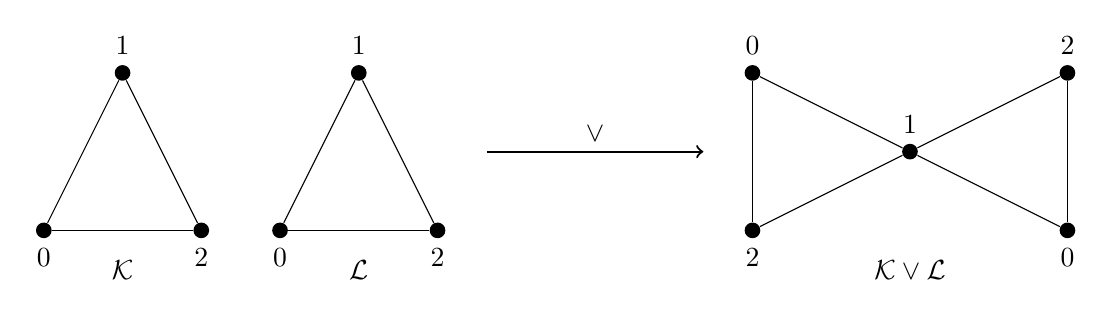
\begin{tikzpicture}
\node[fill=black, circle, inner sep=2pt, label=below:{$0$}] (A) at (0,0) {};
\node[fill=black, circle, inner sep=2pt, label=below:{$2$}] (B) at (2,0) {};
\node[fill=black, circle, inner sep=2pt, label=above:{$1$}] (C) at (1,2) {};
\node[align=center] at (1,-0.5) (label1) {$\mathcal{K}$};

\node[fill=black, circle, inner sep=2pt, label=below:{$0$}] (D) at (3,0) {};
\node[fill=black, circle, inner sep=2pt, label=below:{$2$}] (E) at (5,0) {};
\node[fill=black, circle, inner sep=2pt, label=above:{$1$}] (F) at (4,2) {};
\node[align=center] at (4,-0.5) (label2) {$\mathcal{L}$};

\node[fill=black, circle, inner sep=2pt, label=above:{$0$}] (G) at (9,2) {};
\node[fill=black, circle, inner sep=2pt, label=below:{$2$}] (H) at (9,0) {};
\node[fill=black, circle, inner sep=2pt, label=above:{$1$}] (I) at (11,1) {};
\node[fill=black, circle, inner sep=2pt, label=above:{$2$}] (J) at (13,2) {};
\node[fill=black, circle, inner sep=2pt, label=below:{$0$}] (K) at (13,0) {};
\node[align=center] at (11,-0.5) (label3) {$\mathcal{K} \lor \mathcal{L}$};

\node at (5.5, 1) (AS) {};
\node at (8.5, 1) (AE) {};

\draw (A) -- (B);
\draw (B) -- (C);
\draw (C) -- (A);

\draw (D) -- (E);
\draw (D) -- (F);
\draw (E) -- (F);

\draw (G) -- (I);
\draw (G) -- (H);
\draw (H) -- (I);
\draw (J) -- (K);
\draw (J) -- (I);
\draw (K) -- (I);

\draw [->, thick] (AS) -- node[above] {$\lor$} (AE);
    \end{tikzpicture} 
    \caption{Examples of the wedge of simplicial complexes.}\label{fig:simwe}
\end{figure}

Now consider the complexes $\mathcal{K} = \PowS_{1}(\{0, 1\})$ and $\mathcal{L} = \PowS_1(\{2, 3\})$. The geometric realization of the join $\mathcal{K} \star \mathcal{L}$ of these complexes can be seen in figure \ref{fig:simjo}. From the figure it becomese apperent that $\lVert \mathcal{K} \star \mathcal{L} \rVert$ is homeomorphic to $\mathbb{S}^1$.

  \begin{figure}[h!]
  \centering
  \begin{tikzpicture}
\node[fill=black, circle, inner sep=2pt, label=below:{$0$}] (D) at (1,0) {};
\node[fill=black, circle, inner sep=2pt, label=below:{$1$}] (E) at (2,0) {};
\node[align=center] at (1.5,-1) (label3) {$\mathcal{K}$};

\node[fill=black, circle, inner sep=2pt, label=below:{$2$}] (D) at (2,2) {};
\node[fill=black, circle, inner sep=2pt, label=below:{$3$}] (E) at (3,2) {};
\node[align=center] at (2.5,1) (label3) {$\mathcal{L}$};

\node[fill=black, circle, inner sep=2pt, label=above:{$0$}] (G) at (7,2) {};
\node[fill=black, circle, inner sep=2pt, label=below:{$3$}] (H) at (7,0) {};
\node[fill=black, circle, inner sep=2pt, label=above:{$2$}] (I) at (9,2) {};
\node[fill=black, circle, inner sep=2pt, label=below:{$1$}] (K) at (9,0) {};
\node[align=center] at (8,-0.5) (label3) {$\mathcal{K} \star \mathcal{L}$};

\node at (4, 1) (AS) {};
\node at (6, 1) (AE) {};

\draw (G) -- (H);
\draw (H) -- (K);
\draw (K) -- (I);
\draw (I) -- (G);

\draw [->, thick] (AS) -- node[above] {$\star$} (AE);
  \end{tikzpicture}
  \caption{Example of the join of simplicial complexes.}\label{fig:simjo}
  \end{figure}
\end{ex}

The fact that the join of a two points with two points results in a simplicial complex that has a geometric realization that is homeomorphic does not only work with $\mathbb{S}^1$. This fact holds more generally for the n-fold join of 2-point simplicial complexes. 

\begin{lemma}
  Let $\mathcal{K}_n := \PowS_1(\{(0, n), (1, n)\})$ for $n \in \N^+$, then
  \begin{equation*}
    \left\lVert \bigstar_{i=1}^k \mathcal{K}_i \right\rVert \: \cong \: \mathbb{S}^{k-1}.
  \end{equation*}
\end{lemma}

% TODO: finish proof or search for source of proof
\begin{proof}
  - define $f_n$ realization inductively
  - proof that polyhedra are triangulation of sphere
\end{proof}
